\chapter[Modelling Bilayer Materials]{Modelling Bilayer Materials}
\label{ch:bilayers}

\begin{chapterabstract}
A computationally tractable \mc{} method using triangle rafts is developed to generate bilayers of \sioii{} and related materials.
The method allows defect free networks of any given shape to be grown with both tuneable ring statistics and topologies, controlled by a combination of the ``allowed'' rings and the effective growth ``temperature''. 
Configurations are generated with \aw{} parameters commensurate with those obtained from an analysis of experimental configurations, improving significantly on previous methods.
The ability to efficiently grow configurations allows exploration of the structural basis of \lm’s law, where the commonly observed value of $p_6\approx0.4$ is presented as a balance between entropic and enthalpic factors. 
The deviations of ring areas from the ideal values are discussed and the relative insensitivity of the ring area to relatively strong distortions is highlighted.
\end{chapterabstract}

\section{Bilayer Materials}

An important class of \td{} materials which have emerged in the 21\st{} century are bilayers of silica, \sioii, and related species \cite{Buchner2017}.
The interest in these materials largely stems from the potential to control the structure and pore geometries, with the end goal being to replicate the successes of zeolitic catalysts but in reduced dimensionality. 
Silica bilayers can be prepared experimentally by chemical vapour deposition on metal and graphene supports \cite{Huang2012,Lichtenstein2012a}.
As in the three\--dimensional glass, the basic building blocks of silica bilayers are vertex sharing \sioiv{} tetrahedra, maintaining full coordination for all atoms in the bulk \cite{Wilson2013}.
These are arranged such that three of the vertices are connected to tetrahedra in the same layer, with the final vertex being shared between layers acting as a ``bridge'' (figure \ref{fig:bilayer1}).
A consequence of these bridging oxygen atoms is to enforce a symmetry plane between the upper and lower layers.

Topologically, the symmetry plane means that these materials can be viewed as effective \td{} networks.
Taking one of the layers, without the bridging oxygens, and projecting the atoms onto the horizontal plane reveals a representation of vertex sharing triangles, referred to as a triangle raft (figure \ref{fig:bilayer2}).
The ring structure then emerges from the 3\--coordinate network formed by connecting the silicon atoms of adjacent triangles, as in figure \ref{fig:bilayer3}.
Indeed, a suite of analytical methods, comprising scanning tunnelling microscopy (STM), atomic force microscopy (AFM) and scanning transmission electron microscopy (STEM), have been used to directly visualise the ring structure in silica bilayers, revealing both crystalline and glassy arrangements and even the interface between the two   \cite{Loffler2010,Lichtenstein2012b}.

More recently, experimentalists have also succeeded in synthesising bilayers of aluminosilicates and germania, \geoii{} \cite{Jhang2017,Lewandowski2018,Lewandowski2019}.
The realisation of these materials have posed additional challenges.
The relative difficulty in obtaining bilayers of germania as opposed to silica can be traced back to the inter\--tetrahedal angles.
Whilst silica has a Si\--O\--Si angle of $\sim 150^\circ$, the analogous Ge\--O\--Ge angle is $\sim 130^\circ$ \cite{Neuefeind1996}, a difference which can be attributed to many\--body ion polarisation effects \cite{Wilson2012a,Wilson2012b}.
The consequence of this reduced bond angle is that it is energetically less favourable to adopt the $180^\circ$ tetrahedra required in the bilayer and significant rumpling of the surface is required.

\begin{figure}[bt]
     \centering
     
     \begin{subfigure}[b]{0.3\textwidth}
         \centering
         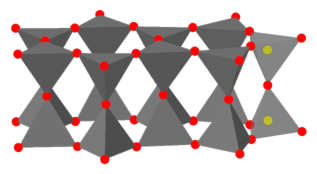
\includegraphics[width=\textwidth]{./figures/bilayers/mx2_bilayer_1.pdf}
         \vspace{-1mm}
         \caption{Tetrahedral bilayer}
         \label{fig:bilayer1}
     \end{subfigure}
     \hfill
	\begin{subfigure}[b]{0.3\textwidth}
         \centering
         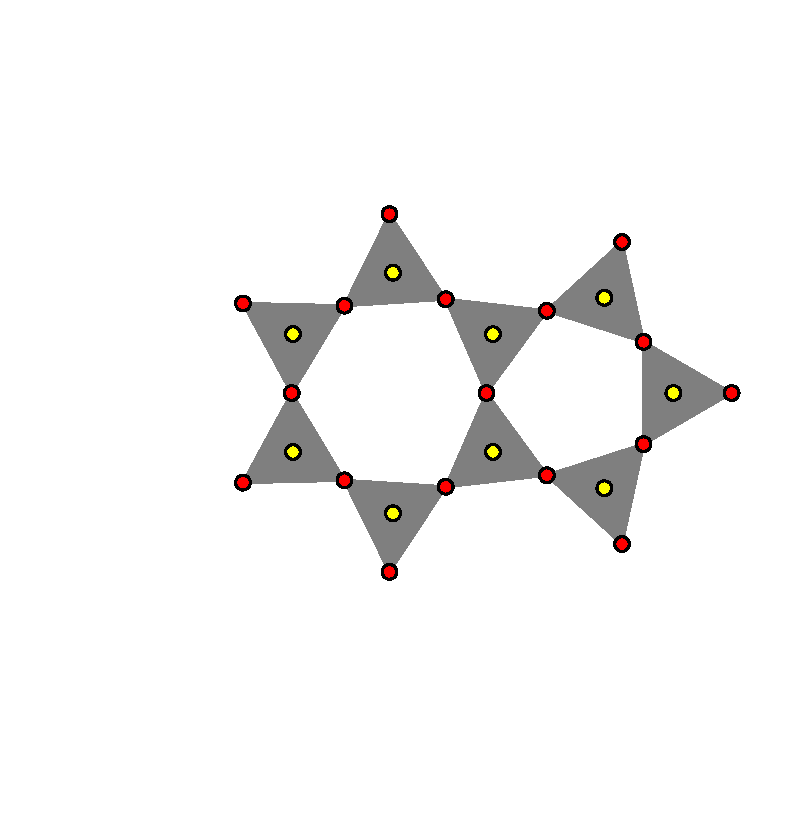
\includegraphics[width=\textwidth]{./figures/bilayers/mx2_bilayer_2.pdf}
         \caption{Triangle raft}
         \label{fig:bilayer2}
     \end{subfigure}
     \hfill
     \begin{subfigure}[b]{0.3\textwidth}
         \centering
         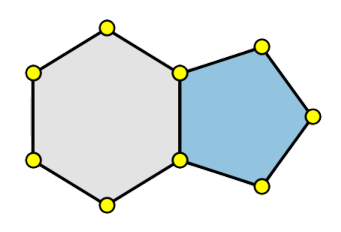
\includegraphics[width=0.8\textwidth]{./figures/bilayers/mx2_bilayer_3.pdf}
         \vspace{5mm}
         \caption{Ring structure}
         \label{fig:bilayer3}
     \end{subfigure}
     \hfill
     
     \caption{Silica bilayers of vertex sharing tetrahedra in panel (a) can be represented as a \td{} triangle raft in panel (b). Silicon and oxygen atoms are coloured yellow and red respectively. The ring structure then emerges from the 3\--coordinate network comprising the silicon atoms, panel (c).}
     \label{fig:bilayer}
\end{figure}

\section{Review of Existing Methods}
\label{s:triraftexisting}

As mentioned in the  introduction, both \abinitio{} methods and classical molecular dynamics have been used in computational studies of silica bilayers, which often require a starting atomistic configuration  \cite{Bjorkman2013,Malashevich2016,Wilson2013,Roy2018}.  
One approach is to simply take an experimental sample as the starting structure. 
Whilst this may be the best solution, the experimental configurations can contain defects or areas where the image is corrupted \ie{} the configuration may not be ``pristine''.
Additionally, the location of each atom has an associated uncertainty which leads to discrepancies in the observed bond lengths and angles, which can be compounded by any out\--of\--plane distortions.
Whilst computational refinement can attenuate these problems \cite{Sadjadi2017,Wilson2018}, there remains the more fundamental question of how ``typical'' the available images are from experiment.
STM and AFM provide exceptionally well resolved information but only on relatively small sample sizes.
Computational techniques can therefore prove a valuable tool for generating a large number of high\--quality configurations and corroborating experimental information.  

One current approach is to transform amorphous graphene configurations \cite{Wilson2013}.
Here disordered networks are generated using a bond switching method (as outlined in section \ref{s:bondswitch}), before the carbon atoms are exchanged for silicon and decorated with oxygens.
Whilst this is a valid approach, the method assumes that the two materials are topologically equivalent.
This is likely an oversimplification, as the presence of the bridging oxygens in silica afford the structure increased flexibility when compared to the carbon analogue.
It also may explain why this method has struggled to mirror experimentally observed values of the ring statistics and \aw{} parameter, with small and large ring proportions being under\--estimated \cite{Kumar2014}.

An alternative approach is to use molecular dynamics coupled with an effective pair potential to obtain viable configurations \cite{Roy2018}.
Such techniques are relatively common, having been employed previously to study amorphous graphene \cite{Kumar2012}. 
These methods offer the potential for generating realistic configurations but are difficult to control as the cooling rates which must be applied are necessarily huge compared to experimental rates. 
A potential artefact of the high cooling rates is the effectively freezing in of defect states, either in terms of local coordination environments or highly\--strained (three-membered) rings.
In addition, as with the method above, such methods appears to systematically underestimate the \aw{} parameter, indicative of too little structural ordering.

\section{Triangle Raft Method}
\label{s:triangleraft}

The motivation of this work was to develop a construction algorithm to generate samples of silica bilayers which can capture the full \td{} network topology, including both the ring distribution \textit{and} correlations. 
The model should be able to explore all phases from crystalline to amorphous yet be computationally efficient enough to produce configurations suitable for further high throughput calculations. 
To achieve this a grow-from-seed Monte Carlo algorithm has been developed, where rings are individually added to build a triangle raft.
This approach takes inspiration from the first hand\--built models, which have traditionally been noted to bear close resemblance to experimental structures \cite{Shackelford1982a,Buchner2016a}.
Such models were superseded by computational techniques designed to generate periodic configurations. 
However, the recent development in techniques to simulate aperiodic samples, such as sliding boundary conditions for molecular dynamics \cite{Theran2015}, makes this constraint no longer essential, and benefit may be gained from the added freedom of an aperiodic model.


\subsection{Potential Model}

As explained in figure \ref{fig:bilayer} it is possible to capture the full topology of silica bilayers with a simplified representation consisting of a network of vertex\--sharing \sioiii{} triangles. 
As the focus of this chapter is on generating a large number of samples with varying ring statistics, %to be used as a base for further calculations, 
working with this reduced representation is sufficient, as it provides a computationally efficient way to produce networks with the required \textit{topology}. 
The precise \textit{geometry} of the bilayer can be refined with advanced optimisation techniques if required \cite{Tangney2002}. 

In order to simulate bilayer systems in two dimensions, a suitable potential model is needed which captures the essential physics of the system: the local triangular environment of the \sioiii{} units and the relative energies of rings of different sizes. 
The model used here is modified from a relatively simple potential used in all\--atom bilayer calculations \cite{Wilson2013,Wilson2018}, a schematic for which is given in figure \ref{fig:trpotmodel}.
Each \sioiii{} unit has a harmonic potential acting between all three Si\---O pairs, and the three nearest\--neighbour O\---O pairs, given by:
\begin{equation}
	\label{eq:harmonic}
	\mathcal{U}_{ij} = \frac{\fk}{2}\left(r_{ij}-r_{ij}^{0}\right)^{2},
\end{equation}
where $\fk$ is a constant, $r_{ij}$ is the interatomic separation and $r_{ij}^{0}$ the equilibrium interatomic separation between $i,j$. 
The spring constant, $\fk$, is set to be very stiff, whilst the equilibrium separations are set according to elemental species such that $r_{\text{OO}}^{0}=\sqrt{3}\,r_{\text{SiO}}^{0}$, maintaining a set of ideal \sioiii{} triangles. 

The Si\---O\---Si angle, which determines the strain associated with different ring sizes, is controlled by a shifted and cut 24\--12 potential of the form:
\begin{equation}
	\mathcal{U}_{ij} = 
	\begin{cases}
	\epsilon \left[ \left(\frac{r_{0}}{r_{ij}}\right)^{24}-2\left(\frac{r_{0}}{r_{ij}}\right)^{12} \right] + \epsilon & r_{ij}\leq r_{0} \\
	0 & \text{otherwise}
	\end{cases}
\end{equation}
where $\epsilon$ is a constant and $r_{ij}$ is now the Si\---Si separation between atoms in adjacent triangles. 
It is the value of $r_{0}$ which sets the Si\---O\---Si angle at which strain begins to be felt and therefore the relative ring energies.
Taking the hexagonal lattice as being the zero in energy it follows that $r_{0}=2r_{\text{SiO}}$.
Rings which deviates increasingly from the ideal hexagon will therefore incur an increasingly energetic penalty.

\begin{figure}[bt]
     \centering
  
         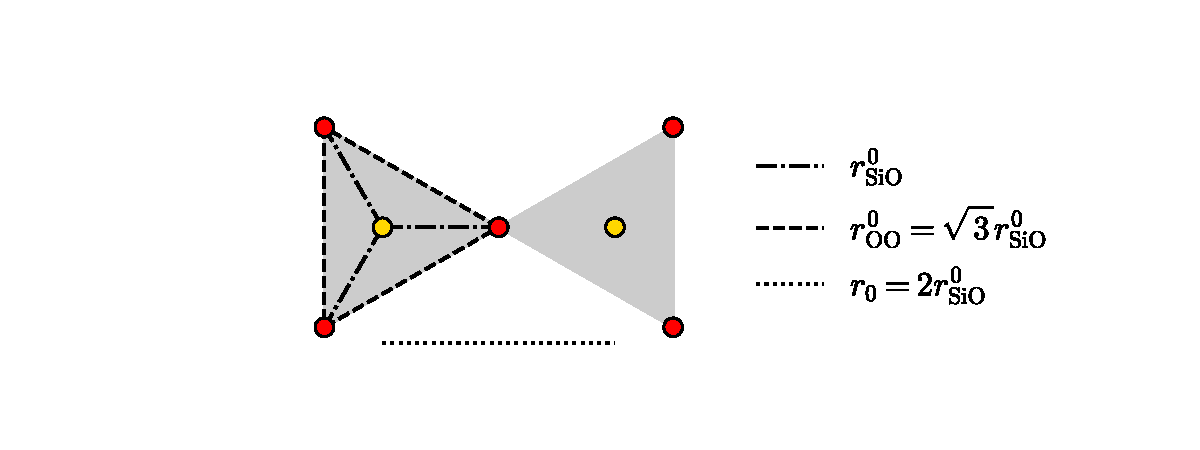
\includegraphics[width=0.6\textwidth]{./figures/bilayers/tr_pot_model.pdf}
 
     \caption{Schematic of the potential model in triangle rafts. Stiff harmonic springs (dashed and dashed\--dotted lines) preserve the triangular subunits, whilst the shifted and cut 24\--12 potential (dotted line) maintains an equilibrium inter\--triangle angle of $120^\circ$ between neighbouring subunits.}
     \label{fig:trpotmodel}
\end{figure}

To summarise, the primary aim here is to generate topologies suitable for later investigation using more detailed (\ie{} more accurate but
computationally\--demanding) potential models. 
As a result, the harmonic springs simply control the triangular geometries whilst the 24-12 potential controls the repulsion between these local units. 
These functions are chosen as deliberately simple to improve computational efficiency and achieve high throughput of idealised networks. 
Furthermore, the parameters $\fk$ and $\epsilon$ need have no direct physical meaning, simply controlling the
meaning of the system ``temperature'' as discussed below. 
The only requirement is that they generate energies of the same magnitude to allow for efficient
structural evolution.


\subsection{Algorithmic Details}


Using the model detailed above, a Monte Carlo construction algorithm has been developed which allows two\--dimensional networks to be built ring by ring in the shape of a specified function. The main steps of the algorithm are outlined below:
\begin{enumerate}
	\item Take a starting seed, such as a single ring or experimental configuration
	\item Select triangles on which to build the next ring (see figure \ref{fig:triraftalgsearch})
		\label{en:loopstart}
		\begin{enumerate}
			\item Overlay a function on the network (\eg{} circle, square)
			\item Check for atoms with dangling bonds lying inside the function region
			\item If no such atoms exist, systematically increase the function size until an atom is found
			\item Find the next nearest atoms which also have a dangling bonds
			\item Choose the two triangles that correspond to the largest starting ring size	
		\end{enumerate}
	\item Determine the probability of constructing rings of different sizes
		\begin{enumerate}
			\item Build trial rings in the range $k_{\text{min}}$ to $k_{\text{max}}$ (see figure \ref{fig:triraftalgtrial})
			\item Geometry optimise the local structure and calculate minimised potential energy (as explained in section \ref{s:geomopt})
			\item Calculate the probabilities of each ring occurring, $P_k$, equation \eqref{eq:probdist}
		\end{enumerate}
	\item Accept single trial ring according to the probability distribution
		\label{en:loopend}
	\item Repeat steps \ref{en:loopstart} $\rightarrow$ \ref{en:loopend} until the target number of rings is reached
\end{enumerate}

\begin{figure}[bt]
     \centering
     
     \begin{subfigure}[b]{0.45\textwidth}
         \centering
         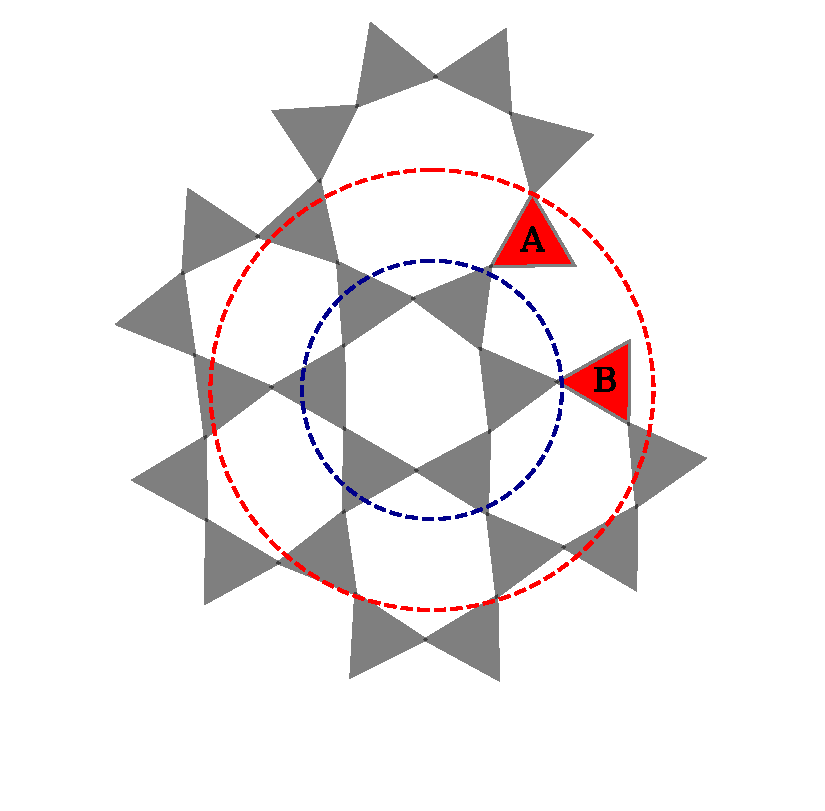
\includegraphics[width=0.5\textwidth]{./figures/bilayers/alg_search_1.pdf}
         \vspace{-1mm}
         \caption{}
         \label{fig:triraftalgsearch1}
     \end{subfigure}
	\begin{subfigure}[b]{0.45\textwidth}
         \centering
         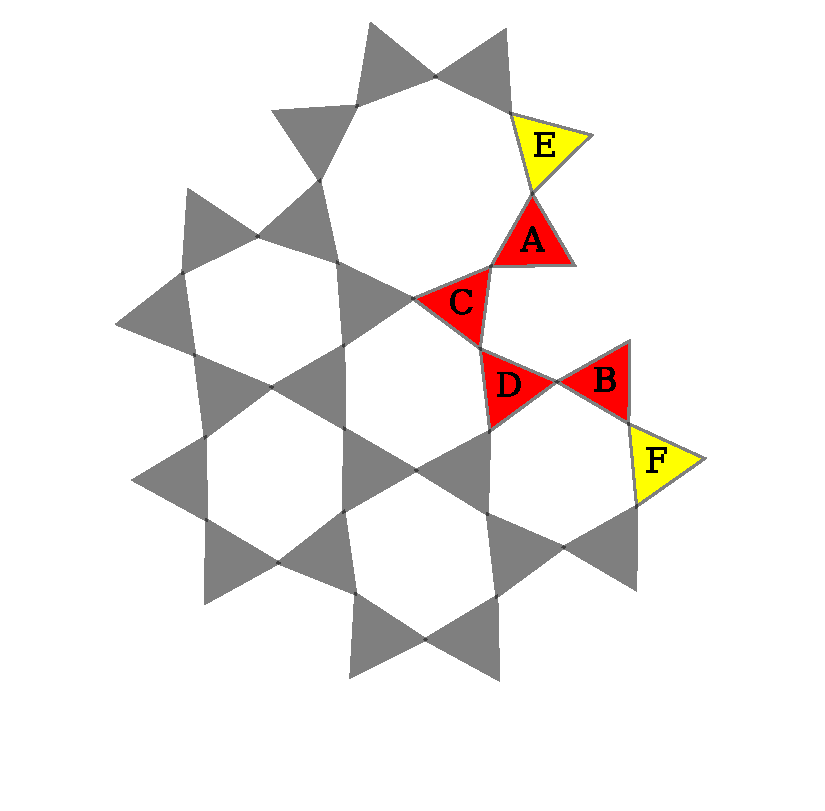
\includegraphics[width=0.5\textwidth]{./figures/bilayers/alg_search_2.pdf}
         \caption{}
         \label{fig:triraftalgsearch2}
     \end{subfigure}
   
     \caption{Panel (a) shows how triangles used to construct a ring are initially selected. There are no atoms with dangling bonds within the first search region (blue dashed line), and so the search area is extended (red dashed line), where triangles A and B are found. Panel (b) gives the three possibilities for the triangles that will form part of the constructed ring: A–C–D–B, A–E, B–F. As A–C–D–B corresponds to the largest starting ring size this is selected.}
     \label{fig:triraftalgsearch}
     
     \vspace{2mm}
     
     \begin{subfigure}[b]{0.18\textwidth}
         \centering
         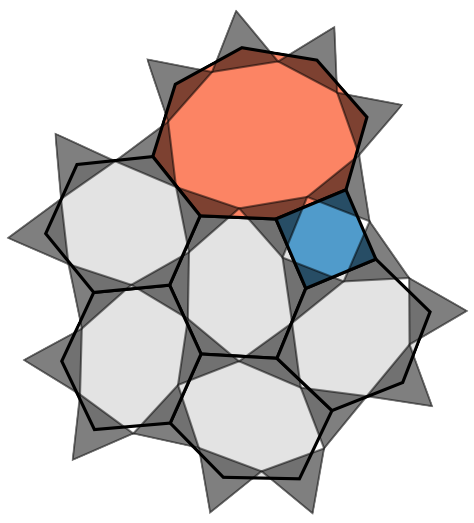
\includegraphics[width=\textwidth]{./figures/bilayers/alg_4.pdf}
         \caption{}
         \label{fig:triraftalgtrial1}
     \end{subfigure}
     \hfill
     \begin{subfigure}[b]{0.18\textwidth}
         \centering
         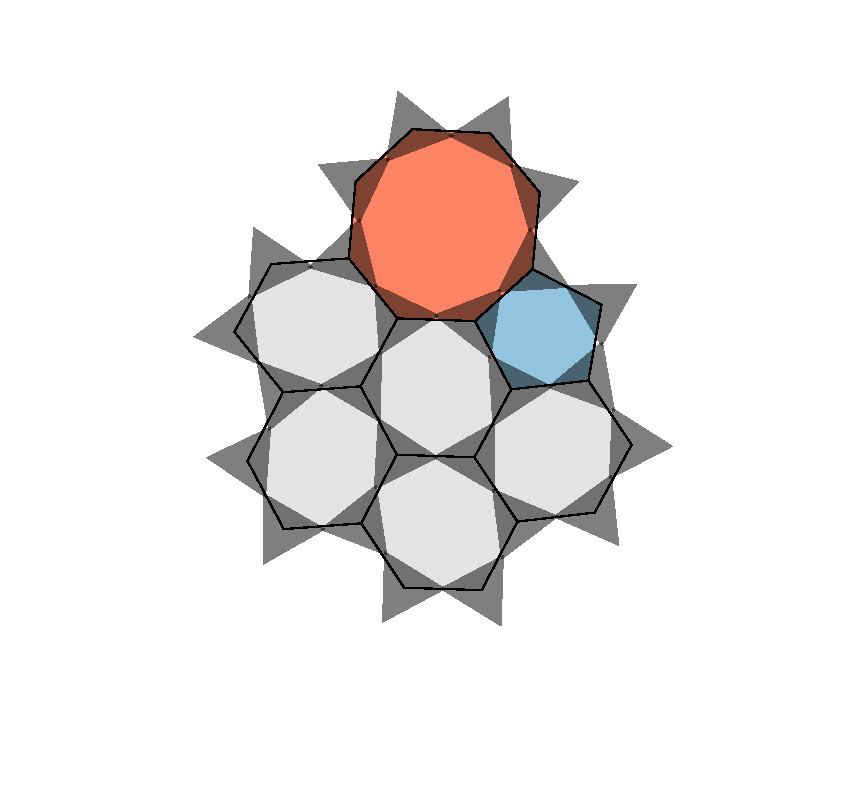
\includegraphics[width=\textwidth]{./figures/bilayers/alg_5.pdf}
         \caption{}
         \label{fig:triraftalgtrial2}
     \end{subfigure}
     \hfill
     \begin{subfigure}[b]{0.18\textwidth}
         \centering
         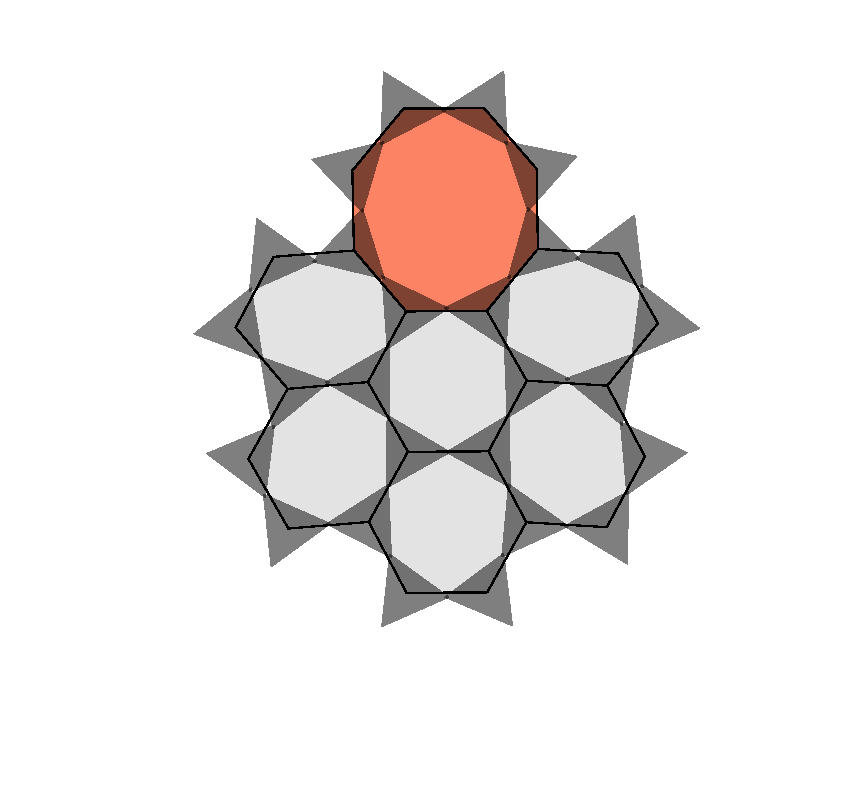
\includegraphics[width=\textwidth]{./figures/bilayers/alg_6.pdf}
         \caption{}
         \label{fig:triraftalgtrial3}
     \end{subfigure}
     \hfill
      \begin{subfigure}[b]{0.18\textwidth}
         \centering
         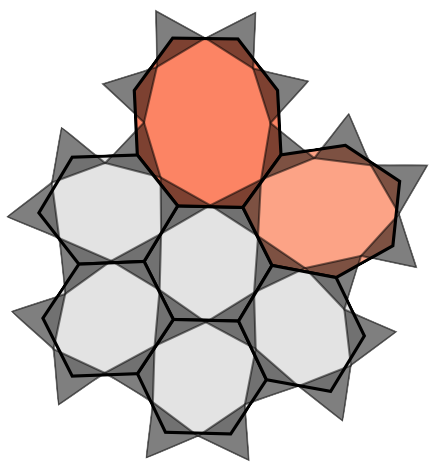
\includegraphics[width=\textwidth]{./figures/bilayers/alg_7.pdf}
         \caption{}
         \label{fig:triraftalgtrial4}
     \end{subfigure}
     \hfill
      \begin{subfigure}[b]{0.18\textwidth}
         \centering
         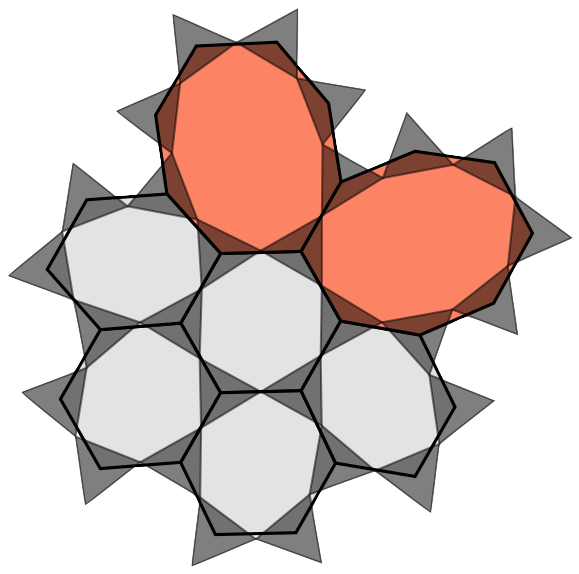
\includegraphics[width=\textwidth]{./figures/bilayers/alg_8.pdf}
         \caption{}
         \label{fig:triraftalgtrial5}
     \end{subfigure}
     \hfill
     \caption{Geometry optimised structures for trial rings in the range $k = 4-8$. The ring structure is shown along with the \sioiii{} triangle.}
     \label{fig:triraftalgtrial}
    
\end{figure}

\noindent The probability of a ring of size $k$ being accepted, $P_k$, is given by the equation:
\begin{equation}
	\label{eq:probdist}
	P_k=\frac{ \exp{\left[-\left(\mathcal{U}_{k}-\mathcal{U}_k\right)/T\right]}}{\sum\limits_{k}\exp{\left[-\left(\mathcal{U}_{k}-\mathcal{U}_{0}\right)/T\right]}},
\end{equation}
where $\mathcal{U}_k$ and $\mathcal{U}_{0}$ correspond to the energy of the trial structure and lowest energy of all trial structures respectively, and $T$ is a ``temperature''. 
The parameter $T$ controls how easily the potential energy landscape can be explored, and therefore how accessible strained rings become. 
In the low $T$ limit, the acceptance probabilities are dominated by the energy term, and the rings which are selected will be those with the lowest energy. 
Note that this is not necessarily the 6-ring, but rather is dependent on the local environment. On the other hand, in the high $T$ limit, the acceptance probabilities are approximately equal, and rings are selected on a more random basis. 
This is demonstrated in table \ref{tab:prob}, using the example configurations from figure \ref{fig:triraftalgtrial}. 
The ``temperature'' parameter is therefore the primary method for controlling the distribution of ring sizes in constructed networks.



\begin{table}[bt]
	\centering
	\caption{Variation of acceptance probabilities with temperature for the configurations in figure \ref{fig:triraftalgtrial}.}
	\label{tab:prob}
	\begin{tabular}{c c c c c c}
	\toprule
	$P_{k}$ & 4 & 5 & 6 & 7 & 8 \\[0.5mm]
	\midrule
	$T=10^{-4}$ & 0.0000 & 1.0000 & 0.0000 & 0.0000 & 0.0000 \\[0.5mm]
	$T=10^{-3}$ & 0.0000 & 0.8837 & 0.1162 & 0.0001 & 0.0000 \\[0.5mm]
	$T=10^{-2}$ & 0.0336& 0.4104 & 0.3351 & 0.1659 & 0.0550 \\[0.5mm]
	$T=10^{-1}$ & 0.1734 & 0.2227 & 0.2183 & 0.2034 & 0.1822 \\[0.5mm]
	$T=10^{0}\;\;$ & 0.1973 & 0.2023 & 0.2018 & 0.2004 & 0.1982 \\[0.5mm] 
	\bottomrule	
	\end{tabular}
\end{table}

\section{Properties of Triangle Rafts}

The triangle raft method is evaluated in terms of its effectiveness in producing configurations which accurately replicate the network properties of experimental silica bilayers \ie{} the ring statistics and \aw{} parameter.
It is also compared against the existing methods introduced in section \ref{s:triraftexisting}, namely generation from amorphous graphene or molecular dynamics.
This is performed in the wider context of systematically varying the model parameters to explore the behaviour of generic networks of this type.

\subsection{Network Growth}
 
\begin{figure}[p]
     \centering
     
     \begin{subfigure}[b]{0.35\textwidth}
         \centering
         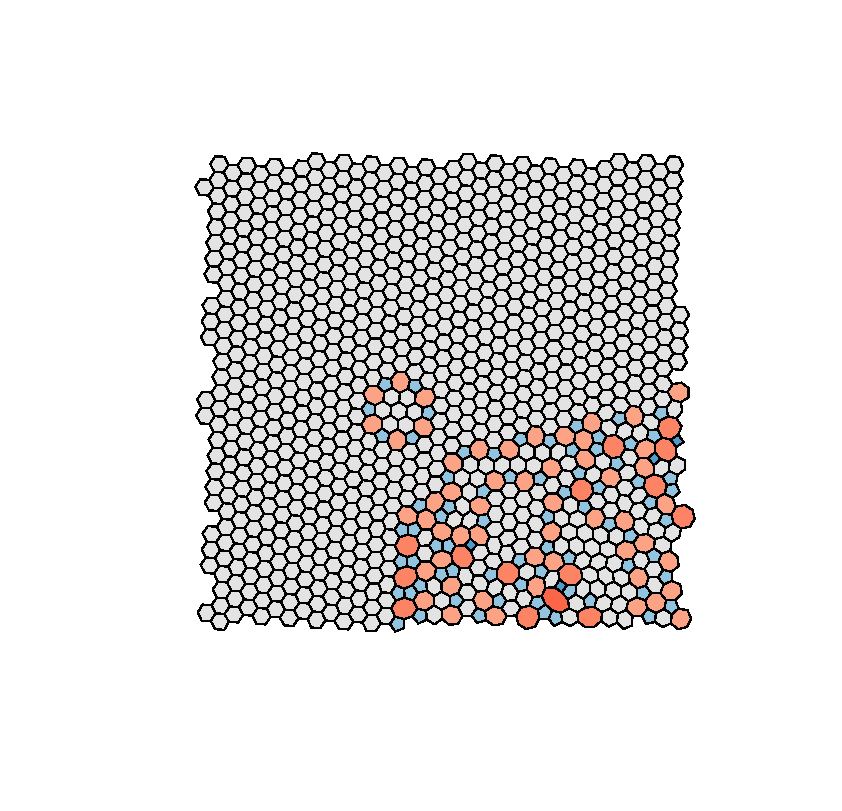
\includegraphics[width=\textwidth]{./figures/bilayers/mx2_sq_1.pdf}
         \caption{}
         \label{fig:triraft1}
     \end{subfigure}
     \hspace{1cm}
     \begin{subfigure}[b]{0.35\textwidth}
         \centering
         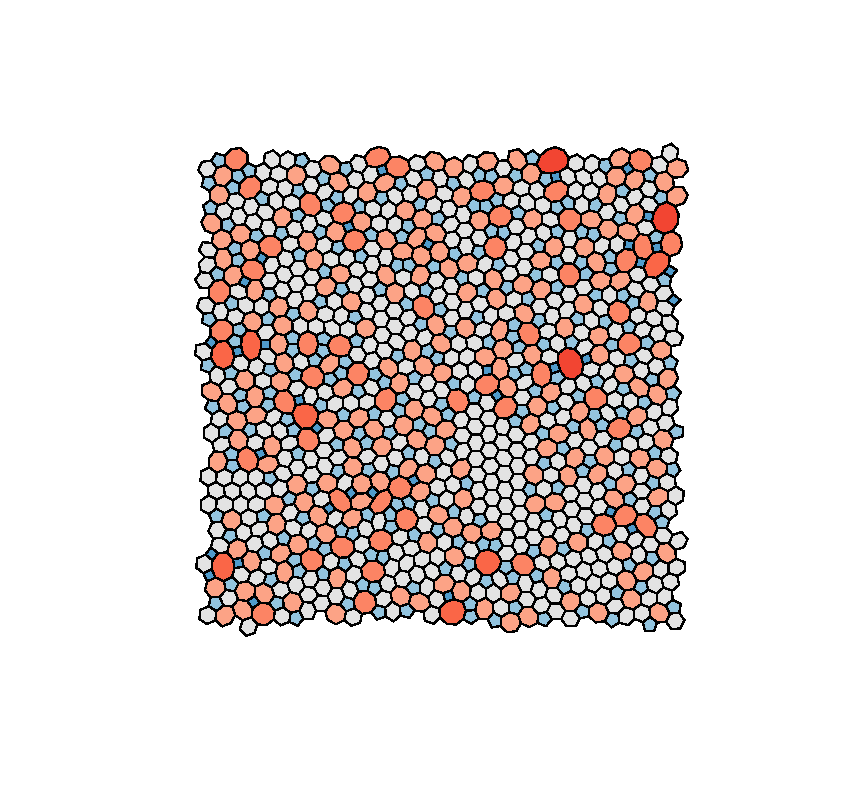
\includegraphics[width=\textwidth]{./figures/bilayers/mx2_sq_2.pdf}
         \caption{}
         \label{fig:triraft2}
     \end{subfigure}
     \hfill
     %\vspace{0.5cm}
     
     \begin{subfigure}[b]{0.35\textwidth}
         \centering
         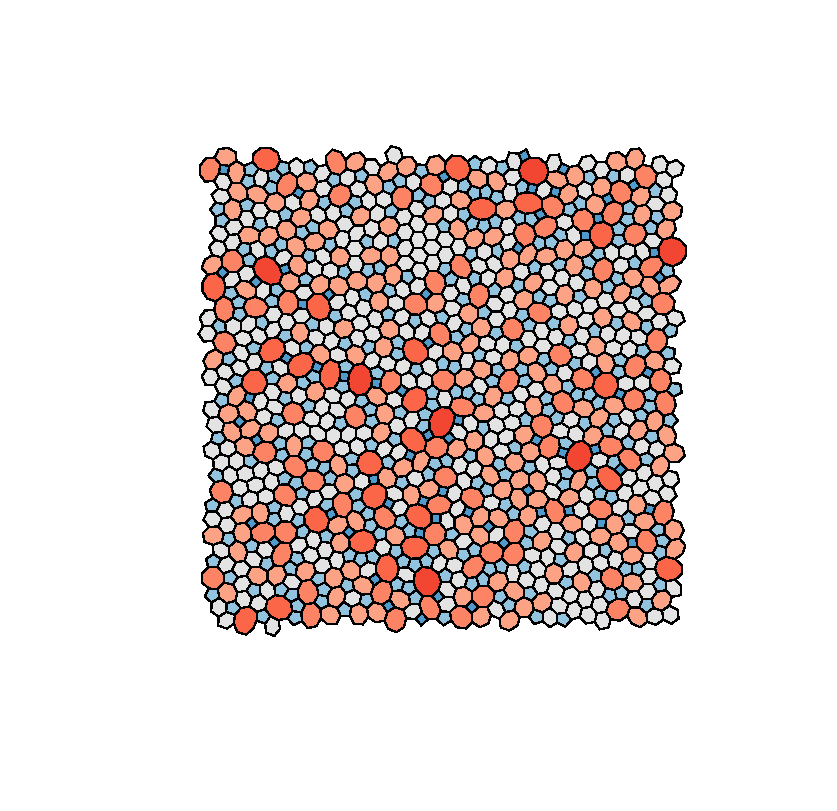
\includegraphics[width=\textwidth]{./figures/bilayers/mx2_sq_3.pdf}
         \caption{}
         \label{fig:triraft3}
     \end{subfigure}
     \hspace{1cm}
      \begin{subfigure}[b]{0.35\textwidth}
         \centering
         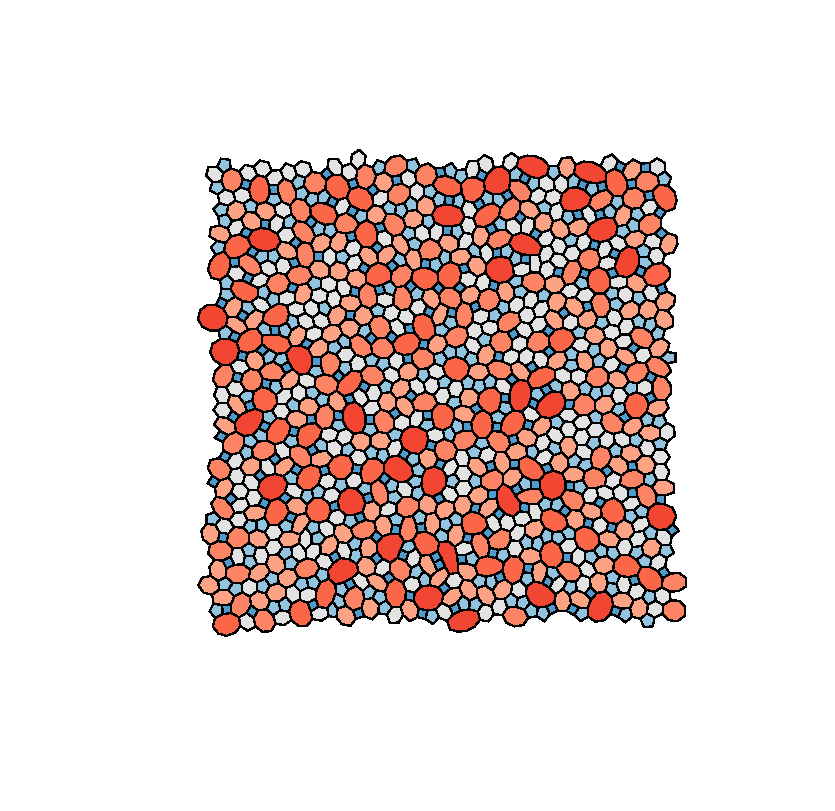
\includegraphics[width=\textwidth]{./figures/bilayers/mx2_sq_4.pdf}
         \caption{}
         \label{fig:triraft4}
     \end{subfigure}
     \hfill
     %\vspace{0.5cm}
     
      \begin{subfigure}[b]{0.35\textwidth}
         \centering
         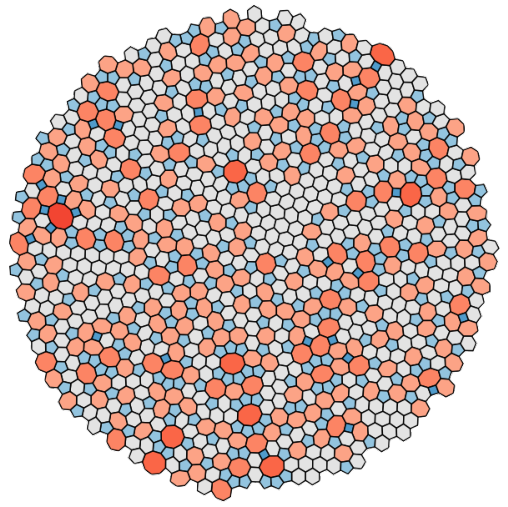
\includegraphics[width=\textwidth]{./figures/bilayers/mx2_circle.pdf}
         \caption{}
         \label{fig:triraft5}
     \end{subfigure}
     \hspace{1cm}
      \begin{subfigure}[b]{0.35\textwidth}
         \centering
         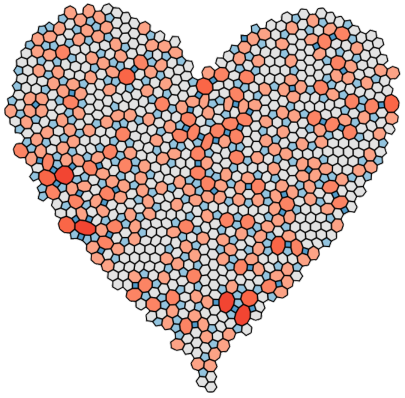
\includegraphics[width=\textwidth]{./figures/bilayers/mx2_heart.pdf}
		\hfill         
         
         \caption{}
         \label{fig:triraft6}
     \end{subfigure}
     
     \caption{Example $1000$ ring configurations generated with different temperatures and shapes. Panels (a) through (d) show square lattices grown at $T=10^{-4.0},\,10^{-3.0},\,10^{-2.5},\, 10^{-2.0}$ respectively. The samples show the increasing diversity in ring structure as temperature is increased. Panels (e) and (f) show configurations with alternative lattice shapes at $T=10^{-3.0}$, demonstrating the flexibility of the method in growing samples with variable geometries. Rings are coloured according to size with $k<6$ as blue, $k=6$ as grey and $k>6$ as red.}
     \label{fig:triraft}
\end{figure} 
 
The triangle raft method is robust and controllable, and is able to generate configurations with tuneable ring statistics and topologies.
Results will largely focus on the system where $k=4\rightarrow10$, denoted $\br{4}{10}$, mimicking the experimentally observed range for silica bilayers. 
Six example configurations are given in figure \ref{fig:triraft}, which are generated with a range of temperatures and growth geometries. 
Figures \ref{fig:triraft1}\--\ref{fig:triraft4} provide a good qualitative analysis of the effect of temperature on the ring structure. 
At low temperature a phase boundary can be seen separating crystalline and amorphous regions, as seen in experimental silica bilayers \cite{Lichtenstein2012b}. 
In these samples although the proportion of small and large rings is low, their positions are highly correlated and chain structures of alternating rings sizes, including the cyclic ``flower'' defect, are clearly present. 
These motifs are reminiscent of defects found in a wide range of materials, including amorphous graphene and thin silicon and germanium oxides \cite{Bjorkman2013,Robertson2012,Buchner2017,Lewandowski2018}. 
In addition, these structural patterns are typical of those found elsewhere in this thesis, in particular chapter \ref{ch:generalnetworks}.
The increase in temperature is coupled with the emergence of rings of more extreme sizes and regions which could be viewed as nano\--crystalline are dispersed. 
The high temperature limit reveals a fully amorphous structure.

Figures \ref{fig:triraft5} and \ref{fig:triraft6} give examples of the diverse geometries in which samples may be constructed. 
It is interesting to note that even ``difficult'' shapes, such as those containing concave regions and cusps, do not prevent growth.  
Although the shape does not affect the network topology (\ie{} does appreciably affect the ring statistics) and is in a sense arbitrary, certain calculations may benefit from the different configurational shapes. 
For instance, molecular dynamics with sliding boundary conditions requires fitting of a smooth function to the sample perimeter, which is facilitated by having a near\--circular form.
Other areas such as percolation problems may benefit from square samples.

\subsection{Network Properties}
\label{s:triraftnetprop}

The quantitative relationship between temperature and ring structure was investigated for three systems of varying ring size ranges;  $\br{5}{7}$, $\br{4}{8}$ and $\br{4}{10}$. 
For each system, 100 samples consisting of 1000 rings were grown at temperatures between $T=10^{-4.5}\rightarrow 10^{-1.5}$. 
The evolution of the combined ring statistics with temperature is presented in figure \ref{fig:trpk}. 
Figures \ref{fig:trpk1}\--\ref{fig:trpk3} give bar representations of the ring size distributions, which show different behaviours. 
For $\br{5}{7}$ the individual $p_k$ are all monotonically increasing ($k\neq 6$) or decreasing ($k=6$) functions, but both $\br{4}{8}$ and $\br{4}{10}$ have $p_k$ containing maxima. 
Additionally, $\br{5}{7}$ and $\br{4}{8}$ achieve uniform distributions in the high temperature limit but not $\br{4}{10}$. 


\begin{figure}[bt]
     \centering
     
     \begin{subfigure}[b]{0.45\textwidth}
         \centering
         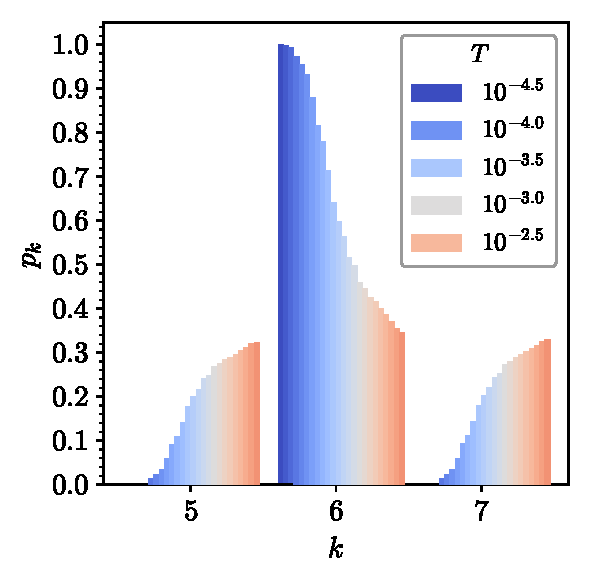
\includegraphics[width=\textwidth]{./figures/bilayers/triraft_57.pdf}
         \caption{$\br{5}{7}$}
         \label{fig:trpk1}
     \end{subfigure}
     \hfill
	\begin{subfigure}[b]{0.45\textwidth}
         \centering
         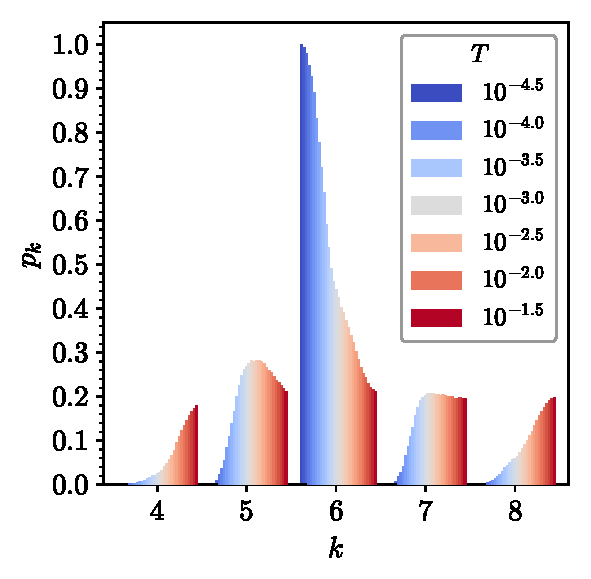
\includegraphics[width=\textwidth]{./figures/bilayers/triraft_48.pdf}
         \caption{$\br{4}{8}$}
         \label{fig:trpk2}
     \end{subfigure}
     \hfill
     
	\vspace{2mm}          
     \begin{subfigure}[b]{0.45\textwidth}
         \centering
         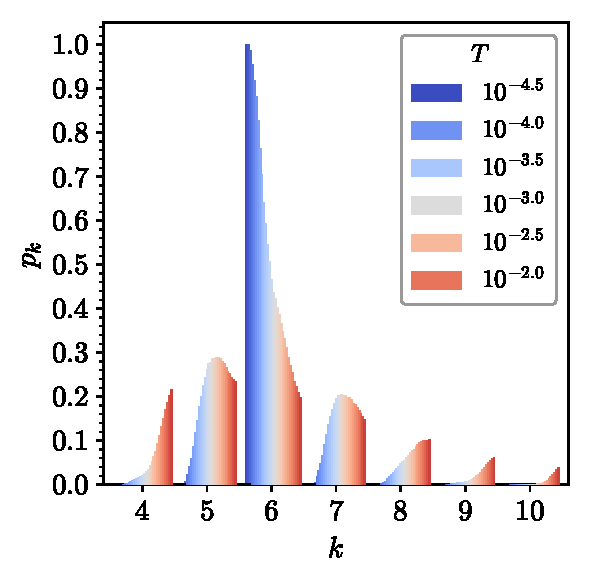
\includegraphics[width=\textwidth]{./figures/bilayers/triraft_410.pdf}
         \caption{$\br{4}{10}$}
         \label{fig:trpk3}
     \end{subfigure}
     \hfill
	\begin{subfigure}[b]{0.45\textwidth}
         \centering
         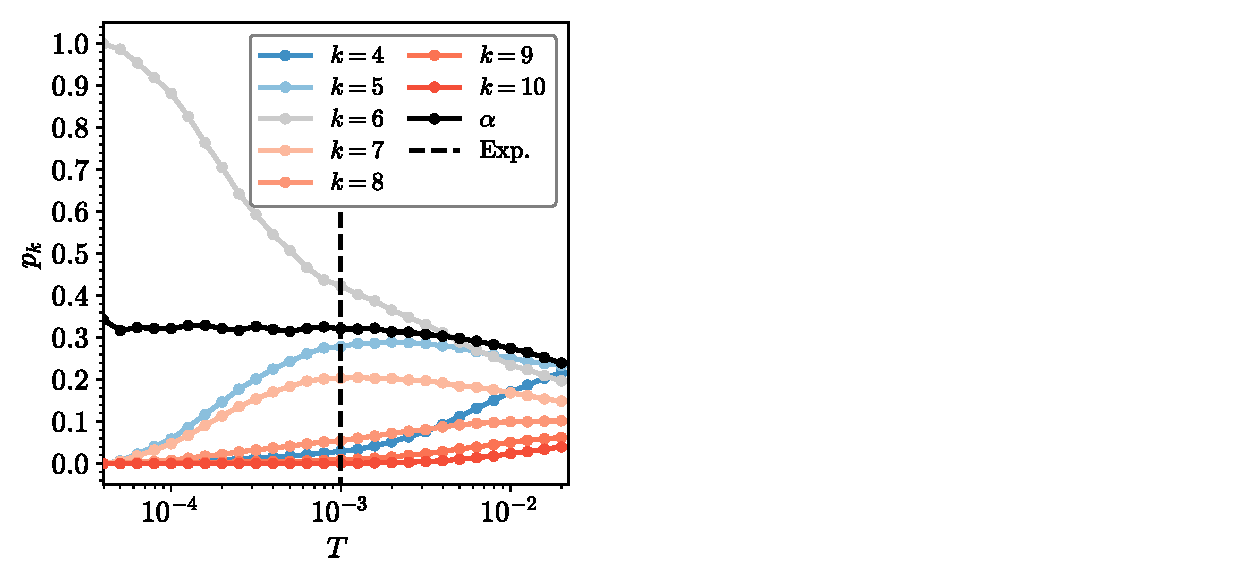
\includegraphics[width=\textwidth]{./figures/bilayers/triraft_line_410.pdf}
         \caption{$\br{4}{10}$}
         \label{fig:trpk4}
     \end{subfigure}
     \hfill
   
     \caption{Variation in ring statistics with temperature over a given allowable $k$\--range. Panels (a)-(c) show bar graph representations of the ring statistics, coloured by temperature, for the $\br{5}{7}$, $\br{4}{8}$ and $\br{4}{10}$ systems. Panel (d) gives an alternative line graph representation of the ring statistics for $\br{4}{10}$, coloured by ring size, along with the Aboav\--Weaire parameter. The temperature which gives the best match to the experimentally observed amorphous region is also highlighted (vertical black dashed line).}
     \label{fig:trpk}
\end{figure}

This disparity in behaviour can largely be traced back to the constraint of Euler's theorem. 
As $\br{5}{7}$ comprises just three ring sizes, Euler's formula demands that $p_5=p_7=\left(1-p_6\right)/2$ and so the system is relatively well defined. 
Hence, because the 5\-- and 7\--rings are more strained than the 6\--ring, $p_5$ and $p_7$ show a systematic increase with temperature. 
Furthermore, the uniform equilibrium distribution can only satisfy Euler's formula when the ring size range is symmetric about 6, as is observed for $\br{5}{7}$ and $\br{4}{8}$. 
The form of the ring statistics at intermediate temperatures and for $\br{4}{10}$ follow the maximum entropy solutions according to \lm's law, discussed in section \ref{s:lemaitre} and later in this section.

The ring distribution for $\br{4}{10}$ is also shown as a function of temperature in figure \ref{fig:trpk4}, along with the value of the \aw{} parameter, $\alpha$, allowing for more facile comparison with experiment. 
The temperature which gives the best agreement to amorphous experimental samples is highlighted by the vertical dashed line. 
The values of $p_k$ and $\alpha$ are provided in table \ref{tab:trpk}, alongside results from two experimental samples. 
It is evident that the model can be successfully tuned to match the topology of the experimental system. 
Not only are the ring distributions in very good accordance, but also the ring correlations, which have until now proved difficult to capture. 
This provides confidence that this simplified but physically motivated triangle raft model is able to reproduce the behaviour of real systems.

Table \ref{tab:trpk} also lists results from previous computational studies which used both Monte Carlo and molecular dynamics methods. 
As mentioned in the review above, neither method fully succeeds in accurately capturing the topology of silica bilayers.
Kumar \etal{} attempted to transform an amorphous graphene structure generated from bond switching \mc{} into a silica bilayer.
The ring statistics of the resulting structure were approximately correct, but the proportion of 5\-- and 6\-- rings over\-- and under\--estimated respectively.
In addition the \aw{} parameter was substantially lower than experiment, indicating a relative lack of structure in the ring ordering.
The origin of these discrepancies is likely the graphene potential model.
The increased stiffness of the carbon network (which unlike silica lacks bridging oxygens) means a high temperature must be used to obtain an amorphous structure with the required disorder.
This leads to heavily distorted rings (as noted in the original paper) which reduces the requirement for small rings to be adjacent to large.


{Roy \etal{} have an alternative approach of generating configurations with an effective pair potential and molecular dynamics.
As can be seen the ring statistics are closer to the experimental values, but now contain artefacts, with a significant fraction of highly strained 3\--membered rings and large rings up to $k=14$.\unskip\parfillskip 0pt \par}


\begin{landscape}
\begin{table}
\centering
\caption{Comparison of silica bilayer samples from experiment, computational modelling and theory.}
\label{tab:trpk}
\begin{threeparttable}
\begin{tabular}{@{}ccccccccccc@{}}
\toprule
& \multicolumn{2}{c}{Experiment} & \phantom{xxx} & \multicolumn{4}{c}{Computation} & \phantom{xxx} & \multicolumn{1}{c}{Theory} \\ 
\cmidrule{2-3} \cmidrule{5-8} \cmidrule{10-10}
& Ru(0001) \cite{Buchner2016a} & Graphene \cite{Huang2012} & & MC\tnote{a}\, \cite{Kumar2014} & MC\tnote{a}\, \cite{Kumar2014} & MD\tnote{b}\, \cite{Roy2018} & TR\tnote{c} & & \lm{} \cite{Gervois1992}  \\ 
\midrule
$N$ & 317    & 444    &&    216 & 418      & $16 \times 85000$ & $1000 \times 100$ && \--- \\ 
$p_3$  &0.0000 & 0.0000 && 0.00 & 0.00     & 0.0038            & 0.0000 && 0.0000 \\ 
$p_4$  &0.0379 & 0.0383 && 0.02   & 0.00     & 0.0537            & 0.0295 && 0.0280 \\  
$p_5$  &0.2744 & 0.2725 && 0.33   & 0.37     & 0.2686            & 0.2786 && 0.2834 \\
$p_6$  &0.4448 & 0.4189 && 0.37   & 0.32     & 0.3773            & 0.4234 &&  0.4200 \\  
$p_7$  &0.1609 & 0.2117 && 0.21   & 0.25     & 0.2224            & 0.2034 && 0.2077 \\  
$p_8$  &0.0757 & 0.0495 && 0.07   & 0.06     & 0.0602            & 0.0544 && 0.0518 \\ 
$p_9$  &0.0063 & 0.0068 && <0.01  & 0.00     & 0.0118            & 0.0097 && 0.0082 \\
$p_{10}$  &0.0000 & 0.0023 && 0.00 & 0.00  & 0.0018            & 0.0010 && 0.0009 \\
$p_{>10}$  &0.0000 & 0.0000 && 0.00 & 0.00 & 0.0004            & 0.0000 && 0.0000 \\ 
$\mu_2$ &  0.9460 & 0.9333 &&  0.94 & 0.86 & 1.1302 & 0.9208 && 0.8985 \\ 
$\alpha$  &0.32   & 0.33 && 0.18 & 0.23 & 0.25 & 0.32 && \--- \\
\bottomrule
\end{tabular}
\begin{tablenotes}
  Note: Each method is given alongside the number of rings in the sample, $N$, followed by the ring statistics, $p_k$, the second moment of the ring statistics, $\mu_2$, and the \aw{} parameter, $\alpha$ \\
  \item[a] Bond switching \mc{} (graphene potential)
  \item[b] Molecular dynamics
  \item[c] Triangle rafts, this work, $T=10^{-3}$
\end{tablenotes}
\end{threeparttable}
\end{table}
\end{landscape}

\noindent These manifest as a result of the artificially high cooling rates in the computational studies which trap defect states in the configurations. 
Once again the final \aw{} parameter, $\alpha$, is underestimated.

It is worth re\--emphasising here that the triangle raft method is able to replicate experimental values of both $p_k$ and $\alpha$, due to its tuneable approach and ``organic'' growth mechanism, where sample formation is not influenced by enforced periodicity. 
Beyond this, the controllable nature of the method also allows insight into key questions% about silica bilayers, 
, for instance the form of the ring distribution in the amorphous phase. 
As detailed in section \ref{s:lemaitre}, the maximum entropy ring distribution can be calculated numerically given the value of $p_6$.
For example, table \ref{tab:trpk} gives the maximum entropy solution for $p_6=0.42$, which agrees very well with the results from triangle rafts and experiment.
This second moment of the distribution, $\mu_2$, is then uniquely related to $p_6$ via \lm's law, shown as the black line in in figure \ref{fig:trlm1}.


\begin{figure}[bt]
     \centering
     
     \begin{subfigure}[b]{0.45\textwidth}
         \centering
         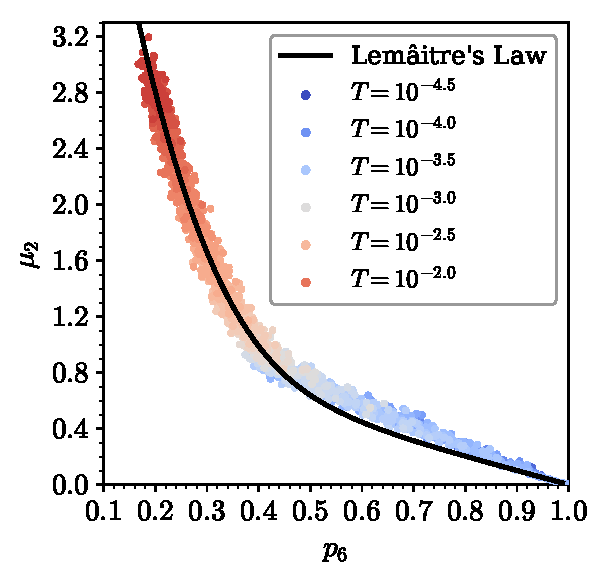
\includegraphics[width=\textwidth]{./figures/bilayers/tri_raft_lm_1.pdf}
         \caption{}
         \label{fig:trlm1}
     \end{subfigure}
     \hfill
     \begin{subfigure}[b]{0.45\textwidth}
         \centering
         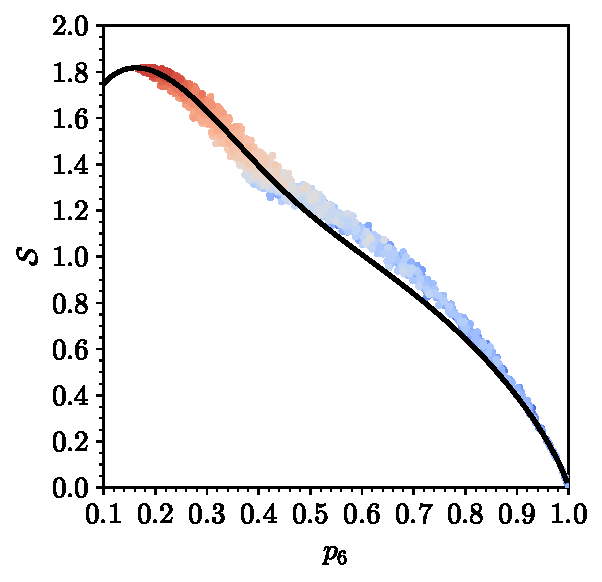
\includegraphics[width=\textwidth]{./figures/bilayers/tri_raft_lm_3.pdf}
         \caption{}
         \label{fig:trlm2}
     \end{subfigure}
     \hfill
     
     \vspace{2mm}
     \begin{subfigure}[b]{0.45\textwidth}
         \centering
         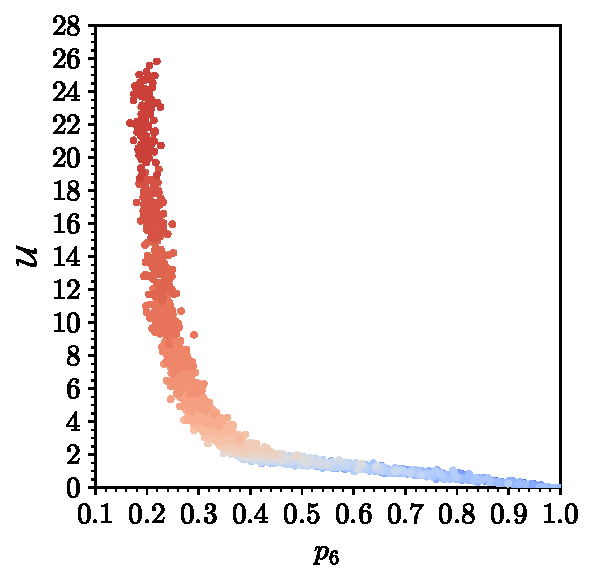
\includegraphics[width=\textwidth]{./figures/bilayers/tri_raft_lm_2.pdf}
         \caption{}
         \label{fig:trlm3}
     \end{subfigure}
     \hfill

     \caption{Evolution of ring statistics, entropy and potential energy (panels (a)-(c)) of triangle rafts with temperature. The experimental value of $p_6\approx 0.4$ occurs just before the exponential increase in potential energy, reflecting the balance of energetic and entropic factors.}
     \label{fig:trlm}
\end{figure}


However, \lm's law gives no information on why a particular maximum entropy distribution is found for a given system.
%The triangle raft method allows systematic generation of configurations with different $p_6$ values by tuning the temperature parameter. 
%The resulting configurations follow \lm's law across the entire temperature range. 
The triangle raft method allows systematic generation of configurations with different $p_6$ values, and the resulting configurations follow \lm's law across the entire range.
Figures \ref{fig:trlm} gives the results from the individual 1000 ring samples, coloured by temperature.
Figures \ref{fig:trlm1} and \ref{fig:trlm2} compare the observed $\mu_2$ and $\mathcal{S}$ (entropy) of the generated configurations to those expected from \lm's law, showing the law provides a good fit, with only a small deviation observed for $p_6>0.5$. 

Figure \ref{fig:trlm3} plots the geometry optimised potential energy of the samples against $p_6$, which increases as the ring sizes become more diverse. 
The curve is split into two regimes, with gradual increase in energy from $p_6=1.0\rightarrow 0.4$ followed by exponential increase for $p_6<0.4$. 
This is consistent with the information in figure \ref{fig:trpk4} which shows that below $p_6\approx 0.4$, not only does the number of extreme ring sizes increase rapidly, but they become less correlated with a lower $\alpha$, decreasing the number of favourable small\--large ring pairings.

It can now be proposed why the experimental amorphous distributions are found with a value of $p_6\approx 0.4$. 
The system aims to maximise entropy by obtaining a ring distribution along the \lm{} curve with the minimum $p_6$ possible. 
However, for $p_6<0.4$ the energetic cost becomes prohibitively large, as higher entropy distributions can only be achieved by increasing the proportion of extreme ring sizes at the expense of relatively low strain 5- and 7- rings.
Interestingly it is also evident why no configurations are present below $p_6\approx 0.16$, even at the highest temperature.
Below this point, the entropy of the $\br{4}{10}$ system decreases whilst the energy continues to rise and so there is no driving force to sample this area of phase space.

\subsection{Physical Properties}
\label{s:trphysprop}

As an additional check that the developed triangle raft model behaves physically, 
the angle distribution between adjacent \sioiii{} units, $f\left(\theta\right)$, was calculated for the $\br{4}{10}$ system across the range of temperatures studied. 
The results are summarised in figure \ref{fig:trang}. 
The angle distributions are necessarily symmetric about $120^\circ$, as each triangle pair contributes two complementary angles. 
At lower temperatures the distribution is dominated by angles close to $120^\circ$, as a consequence of the large proportion of near strainless six membered rings.
Furthermore, at the temperature corresponding to the amorphous experimental region, $T=10^{-3}$, the distribution has a similar extent to the angle distribution found in experimental samples (see for example figure 7 reference \cite{Roy2018}). 
However, as the temperature increases, the form of $f\left(\theta\right)$ does not simply broaden as might be expected, but becomes bimodal. 
This can be rationalised by considering the angles that would be present in regular polygons of different sizes, marked by vertical lines in figure \ref{fig:trang}.  These ideal angles are clustered away from the mean value of $120^\circ$, and hence increasing the diversity of ring sizes through temperature acts to shift the most commonly observed angles from the central value of $120^\circ$. 
It is therefore interesting to note that increasing structure in the angle distribution does not necessarily translate to increased order in the atomic configurations.

\begin{figure}[bt]
     \centering
     
     \begin{subfigure}[b]{0.45\textwidth}
         \centering
         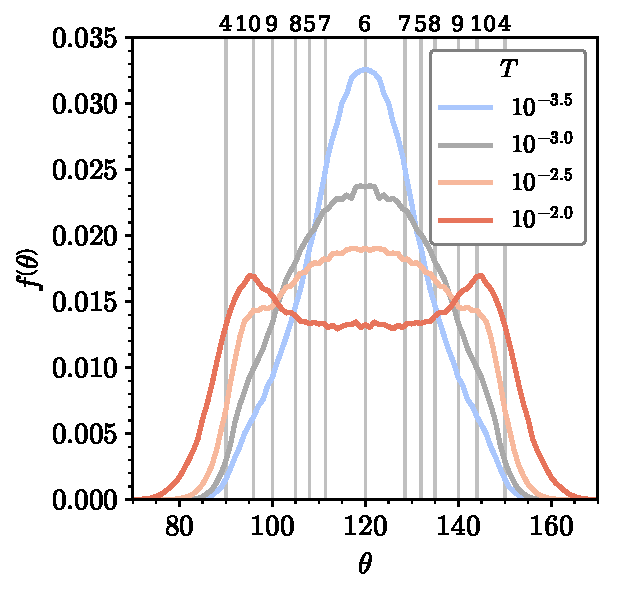
\includegraphics[width=\textwidth]{./figures/bilayers/tri_raft_angle.pdf}
         \caption{}
         \label{fig:trang}
     \end{subfigure}
     \hfill
     
     \begin{subfigure}[b]{0.45\textwidth}
         \centering
         \includegraphics[width=\textwidth]{./figures/bilayers/tri_raft_area.pdf}
         \caption{}
         \label{fig:trarea}
     \end{subfigure}
     \hfill
     \begin{subfigure}[b]{0.45\textwidth}
         \centering
         
\includegraphics[width=\textwidth]{./figures/bilayers/ellipse_area.pdf}
         \caption{}
         \label{fig:trellipse}
     \end{subfigure}
     \hfill

     \caption{Panel (a) gives the ring angle distribution function for triangle rafts formed at different temperatures. Panel (b) compares the regularity of rings in computational and experimental amorphous configurations, with points indicating the mean value and bars corresponding to the standard deviation. Experimental data is taken from ref. \cite{Kumar2014}. Panel (c) shows the effect on the area when distorting a circle to an ellipse whilst maintaining a constant perimeter length.}
     \label{fig:trangarea}
\end{figure}

A final check comes from examining the ring areas in the generated configurations.
Inspection of amorphous experimental samples reveals that the rings appear highly regular in shape. 
This can be quantified by determining the average dimensionless area for each ring size, $A_k$, and comparing it to the area of the corresponding regular polygon, $A_k^0$, where:
\begin{align}
	A_k &= \frac{\langle Area\left(k\right) \rangle}{\left(r_{\text{SiSi}}^{0}\right)^2}, \label{eq:trarea} \\[0.5em]
	A_k^0 &= \frac{k}{4\tan\left(\pi / k \right)} \label{eq:trarea0}.
\end{align}
As the regular polygon has the maximum achievable area for a given ring size, the ratio $A_k / A_k^0$ is expected to lie in the range $0\rightarrow 1$, with a lower value corresponding to increased deviation from regularity, and assuming $r_{\text{SiSi}}^{0}$ to be fixed.

The study by Kumar \etal{} found that whereas for experimental configurations, $A_k / A_k^0 \approx 1$, configurations generated using their bond switching method generally displayed ratios much less than unity \cite{Kumar2012}, indicative of large distortions in the ring structure. 
For larger rings, a value of $A_k / A_k^0 > 1$ was also found, which can only be achieved if there is appreciable bond stretching (see equations \eqref{eq:trarea} and \eqref{eq:trarea0}). 

The analogous results for the method presented in this chapter can be found in figure \ref{fig:trarea}, for $T=10^{-3}$. 
This figure demonstrates that there is now good agreement between experimental and computational results. 
In both cases the deviation from regularity increases with ring size, as the flexibility of the rings increases. 
Again it can be proposed that the difference between current and previous methods could be due to the lack of enforced periodicity on the system. 
By allowing the network to grow relatively freely, the system can avoid a build up of strain associated with maintaining periodic boundaries.

Even with this analysis, an argument can be made that by visual inspection the rings in the experimental configurations are still more regular than those generated from computational samples. 
Therefore one can consider if deformation of a ring should be expected to lead to significant reduction in area. 
This can be explored by considering the distortion of a circle to an ellipse. 
The degree of distortion can be described by the eccentricity of the ellipse,
\begin{equation}
	\xi = \left(1-\frac{b^2}{a^2}\right)^{1/2},
\end{equation}
where $a,b$ are the major and minor axis radii respectively. 
This change in area with distortion is shown in figure \ref{fig:trellipse}, the calculation of which can be found in appendix \ref{app:derivellipse}. 
As can be seen, a large degree of eccentricity is needed for a significant change in the observable area. 
For example, if $a=1.5 b$, the area is still $\approx0.94\%$ of the area of the corresponding circle. 

For silica networks the Si\---Si distances lie in a narrow range because of the nature of the atomic bonding and the near\--linear Si-O-Si bridges
which join the two layers. 
Hence we would expect similar behaviour to occur, with ring areas relatively invariant to distortions in the ring shape (this same analysis would not be expected to hold for foams for example, where the length of the boundary is much more flexible). 
This suggests that the ring area is not the most suitable metric for quantifying the regularity of rings in systems such as this, and could explain any disagreement between the seemingly near ideal ring areas and the visual evidence. 
As previously stated, although the potential model used is physically motivated, it is lightweight in order to facilitate generation of a large number of configurations with the correct network topology. 
In future it would be informative to see if the required regularity can be achieved by geometry optimising the resulting bilayer configurations with a more accurate potential, such as the TS potential which includes potentially significant electrostatic interactions including many-body polarisation effects \cite{Tangney2002}.

\section{Chapter Conclusions}

A method has been developed for effective modelling of silica bilayers and related materials.
Bilayers are represented as triangle rafts, which are sequentially constructed from a seed using a stochastic growth algorithm.
The algorithm is flexible, allowing control over the ring size distribution and overall system topology.
The success of triangle rafts in modelling silica bilayers has been demonstrated by the values of the \aw{} parameter, $\alpha$, which are are more commensurate with those obtained from experimental imaging than configurations generated by previous methods.
Moreover, consideration of the ring areas shows that triangle raft configurations contain highly regular polygons - another experimental observation that has proved challenging to previously capture.

The real advantage of the method is that it enables a computationally tractable and systematic exploration of bilayer systems at increasing levels of disorder.
This has been employed in this chapter for a detailed analysis of \lm's
law, which rationalised why the fraction of six-membered rings observed
in real systems is often $\approx$0.4. 
However, it will also be used in chapter \ref{ch:ph} to investigate the use of persistent homology in amorphous materials.
The ability to build a triangle raft from any user\--defined starting seed also opens further possibilities for the method.
In particular, it would be interesting to see how network growth is affected by the presence of a template, which could be for example a very large ring.
This could lead to insight into how to control pore geometries in these materials.




